% Intended LaTeX compiler: pdflatex
\documentclass[11pt]{article}
\usepackage[utf8]{inputenc}
\usepackage[T1]{fontenc}
\usepackage{graphicx}
\usepackage{longtable}
\usepackage{wrapfig}
\usepackage{rotating}
\usepackage[normalem]{ulem}
\usepackage{amsmath}
\usepackage{amssymb}
\usepackage{capt-of}
\usepackage{hyperref}
\author{Construção de compiladores I}
\date{}
\title{Derivadas e Análise Léxica}
\hypersetup{
 pdfauthor={Construção de compiladores I},
 pdftitle={Derivadas e Análise Léxica},
 pdfkeywords={},
 pdfsubject={},
 pdfcreator={Emacs 28.2 (Org mode 9.7)}, 
 pdflang={English}}
\begin{document}

\maketitle
\section*{Objetivos}
\label{sec:org175b89c}

\subsection*{Objetivos}
\label{sec:org7abad6a}

\begin{itemize}
\item Apresentar outra técnica para obtenção de AFDs
a partir de ERs: derivadas.

\item Apresentar o gerador de analisadores léxicos para Haskell: Alex.
\end{itemize}
\section*{Derivadas de ERs}
\label{sec:org25c4c7b}

\subsection*{Derivadas de ERs}
\label{sec:org7cbee1f}

\begin{itemize}
\item Definição de derivada de uma linguagem:
\end{itemize}

\begin{array}{lcl}
\partial_{a}(L) & = & \{y \in \Sigma^*\,|\,ay \in L\}\\
\end{array}
\subsection*{Derivadas de ERs}
\label{sec:orgdbc2456}

\begin{itemize}
\item Exemplo:
\end{itemize}

\begin{array}{lc}
\partial_{0}(\{10,\lambda,0,01\}) & = \\
 \{\lambda,1\}\\
\end{array}
\subsection*{Derivadas de ERs}
\label{sec:org58ce948}

\begin{itemize}
\item A operação de derivada pode ser definida sobre ERs.
\begin{itemize}
\item Definição da derivada é apenas uma função recursiva.
\end{itemize}
\end{itemize}
\subsection*{Derivadas de ERs}
\label{sec:org0b00492}

\begin{itemize}
\item Operação auxiliar: anulabilidade.
\end{itemize}

\begin{array}{lcl}
\nu(\emptyset)  & = & \bot\\
\nu(\lambda)    & = & \top\\
\nu(a)          & = & \bot\\
\nu(e_1 + e_2)  & = & \nu(e_1) \lor \nu(e_2)\\
\nu(e_1\,e_2)   & = & \nu(e_1)\land \nu(e_2)\\
\nu(e_1^*)      & = & \top\\
\end{array}
\subsection*{Derivadas de ERs}
\label{sec:orgf1b002b}

\begin{itemize}
\item Definição da derivada
\end{itemize}

\begin{array}{lcl}
\partial_{a}(\emptyset)  & = & \emptyset \\
\partial_{a}(\lambda) & = & \emptyset \\
\partial_{a}(a)       & = & \lambda \\
\partial_{a}(b)       & = & \emptyset\,\,\textrm{se }a \neq b\\
\end{array}
\subsection*{Derivadas de ERs}
\label{sec:org1a2245f}

\begin{itemize}
\item Definição de derivada (continuação)
\end{itemize}

\begin{array}{lcl}
\partial_{a}(e_1 + e_2) & = & \partial_a(e_1)+\partial_a(e_2)\\
\partial_{a}(e_1\,e_2)  & = & \partial_{a}(e_1)\,e_2 + \partial_{a}(e_2),\:\:\textrm{se }\nu(e_1) = \top\\
\partial_{a}(e_1\,e_2)  & = & \partial_{a}(e_1)\,e_2\:\:\textrm{se }\nu(e_1) = \bot\\
\partial_{a}(e_1^*)     & = & \partial_{a}(e_1)\,e_1^*\\
\end{array}
\subsection*{Derivadas de ERs}
\label{sec:orge42148f}

\begin{itemize}
\item Número de derivadas é finito sobre uma ER \(e\) é finito.
\begin{itemize}
\item Se considerarmos a equivalência de ER
\end{itemize}
\end{itemize}
\subsection*{Derivadas de ERs}
\label{sec:org8e1c013}

\begin{itemize}
\item Equivalência de ERs
\end{itemize}

\begin{array}{cc}
   e + (e' + e'') \approx (e + e') + e'' & e + e \approx e \\
   e + e' \approx e' + e & (ee')e'' \approx e(e'e'') \\
   \emptyset e \approx \emptyset & e \emptyset \approx \emptyset \\
   e \lambda \approx e  & \lambda e \approx e \\
   e + \emptyset \approx e & \emptyset + e \approx e\\
\end{array}
\subsection*{Derivadas de ERs}
\label{sec:orgae76817}

\begin{itemize}
\item Exemplo: Cálculo da derivada de \((01)^*\).
\end{itemize}

\begin{array}{lc}
  \partial_0((01)^*) & = \\
  \partial_0(01)(01)^* & = \\
  \partial_0(0)1(01)^* & = \\
  \lambda 1(01)^* & = \\
   1(01)^* \\
\end{array}
\subsection*{Derivadas de ERs}
\label{sec:org3d8aceb}

\begin{itemize}
\item Processando strings usando derivadas.
\end{itemize}

\begin{array}{lcl}
\widehat{\partial}(e,\lambda) & = & \nu(e)\\
\widehat{\partial}(e,ay)      & = & \widehat{\partial}(\partial_{a}(e),y)\\
\end{array}
\subsection*{Derivadas de ERs}
\label{sec:orgd29751e}

\begin{itemize}
\item Além de processar palavras diretamente, podemos construir AFDs diretamente
a partir de uma ER.
\end{itemize}
\subsection*{Derivadas de ERs}
\label{sec:org916defe}

\begin{itemize}
\item O AFD correspondente a uma ER \(e\) é: \((E,\Sigma,\delta,e,F)\).
\begin{itemize}
\item \(E\): conjunto de derivadas
\item \(\delta(e,a) = e'\) se \(\partial_{a}(e) = e'\).
\item \(F = \{e\,|\, \nu(e) = \top\}\).
\end{itemize}
\end{itemize}
\subsection*{Derivadas de ERs}
\label{sec:org0376109}

\begin{itemize}
\item Exemplo: Construir um AFD para \((01)^*\).
\begin{itemize}
\item Já calculamos: \(\partial_{0}((01)^*) = 1(01)^*\).
\item \(\partial_{1}((01)^*) = \emptyset\).
\end{itemize}
\end{itemize}
\subsection*{Derivadas de ERs}
\label{sec:org61ac2c9}

\begin{center}
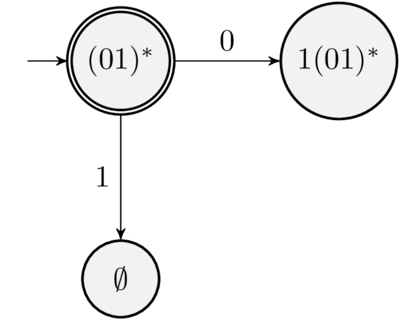
\includegraphics[width=.9\linewidth]{./imgs/image1.png}
\end{center}
\subsection*{Derivadas de ERs}
\label{sec:org78b7014}

\begin{itemize}
\item Repetindo o processo para outras ERs.
\begin{itemize}
\item \(\partial_{0}(\emptyset) = \partial_{1}(\emptyset) = \emptyset\).
\end{itemize}
\end{itemize}

\begin{center}
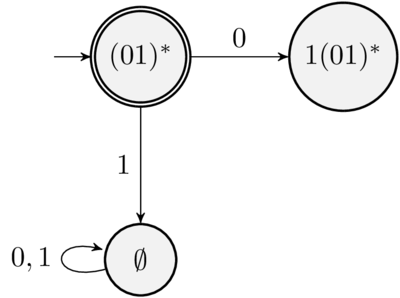
\includegraphics[width=.9\linewidth]{./imgs/image2.png}
\end{center}
\subsection*{Derivadas de ERs}
\label{sec:org03a8a90}

\begin{itemize}
\item Repetindo o processo para outras ERs.
\begin{itemize}
\item \(\partial_{0}(1(01)^*) = \emptyset\).
\item \(\partial_{1}(1(01)^*) = (01)^*\).
\end{itemize}
\end{itemize}

\begin{center}
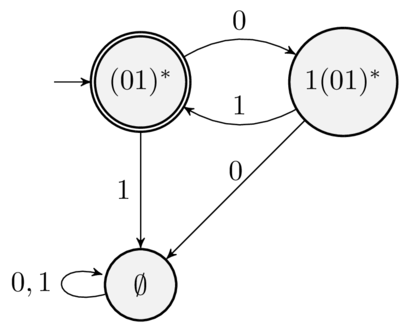
\includegraphics[width=.9\linewidth]{./imgs/image3.png}
\end{center}
\section*{Derivadas em Haskell}
\label{sec:org6821937}

\subsection*{Derivadas em Haskell}
\label{sec:org6cd7e67}

\begin{itemize}
\item Derivadas são de implementação imediata em Haskell.
\end{itemize}
\subsection*{Derivadas em Haskell}
\label{sec:org610f93b}

\begin{itemize}
\item Teste de anulabilidade.
\end{itemize}

\begin{verbatim}
nullable :: Regex -> Bool
nullable Empty = False
nullable Lambda = True
nullable (Chr _) = False
nullable (e1 :+: e2)
  = nullable e1 || nullable e2
nullable (e1 :@: e2)
  = nullable e1 && nullable e2
nullable (Star e1) = True
\end{verbatim}
\subsection*{Derivadas em Haskell}
\label{sec:org3c2e015}

\begin{itemize}
\item Antes de apresentar a função de cálculo de derivadas, é interessante
introduzir algumas funções para realizar simplificações.
\end{itemize}
\subsection*{Derivadas em Haskell}
\label{sec:orgd557451}

\begin{itemize}
\item Simplificando união.
\end{itemize}

\begin{verbatim}
(.+.) :: Regex -> Regex -> Regex
Empty .+. e' = e'
e .+. Empty  = e
e .+. e'     = e :+: e'
\end{verbatim}
\subsection*{Derivadas em Haskell}
\label{sec:org24a3335}

\begin{itemize}
\item Simplificando concatenação
\end{itemize}

\begin{verbatim}
(.@.) :: Regex -> Regex -> Regex
Empty .@. _ = Empty
_ .@. Empty = Empty
Lambda .@. e' = e'
e .@. Lambda = e
e .@. e' = e :@: e'
\end{verbatim}
\subsection*{Derivadas em Haskell}
\label{sec:org3772494}

\begin{itemize}
\item Simplificando o fecho de Kleene.
\end{itemize}

\begin{verbatim}
star :: Regex -> Regex
star Empty = Lambda
star (Star e) = e
star e = Star e
\end{verbatim}
\subsection*{Derivadas em Haskell}
\label{sec:orgd731e90}

\begin{itemize}
\item Definição da derivada
\end{itemize}

\begin{verbatim}
deriv :: Char -> Regex -> Regex
deriv _ Empty  = Empty
deriv _ Lambda = Empty
deriv a (Chr b)
  | a == b = Lambda
  | otherwise = Empty
deriv a (e1 :+: e2)
  = deriv a e1 .+. deriv a e2
deriv a (e1 :@: e2)
  | nullable e1 = deriv a e1 .@. e2 .+. deriv a e2
  | otherwise   = deriv a e1 .@. e2
deriv a (Star e1)
  = deriv a e1 .@. (star e1)
\end{verbatim}
\subsection*{Derivadas em Haskell}
\label{sec:org26a6568}

\begin{itemize}
\item Aceitando uma string.
\end{itemize}

\begin{verbatim}
match :: Regex -> String -> Bool
match e [] = nullable e
match e (c : cs) = match (deriv c e) cs
\end{verbatim}
\section*{Uso do gerador Alex}
\label{sec:org4fc3994}

\subsection*{Uso do gerador Alex}
\label{sec:org2f753d5}

\begin{itemize}
\item A construção de um analisador léxico é uma tarefa automatizável.
\end{itemize}
\subsection*{Uso do gerador Alex}
\label{sec:org2cb624d}

\begin{itemize}
\item Veremos como usar a ferramenta Alex para construir um analisador a partir de uma especificação.
\begin{itemize}
\item Especificações Alex são apenas expressões regulares.
\end{itemize}
\end{itemize}
\subsection*{Uso do gerador Alex}
\label{sec:orgc20de71}

\begin{itemize}
\item Para exemplificar o uso do Alex, vamos considerar uma linguagem de expressões.
\end{itemize}

\begin{array}{lcl}
e & \to  & n \,|\,v\,|\, e + e \,|\, e * e\, (e)\\
\end{array}
\subsection*{Uso do gerador Alex}
\label{sec:orgbd0a4a0}

\begin{itemize}
\item A sintaxe da linguagem de expressões aritméticas é formada pelos seguintes tokens:
\begin{itemize}
\item Números: \emph{n}
\item Variáveis: \emph{v}
\item Símbolos: \emph{+}, \emph{*}, \emph{(} e \emph{)}.
\end{itemize}
\end{itemize}
\subsection*{Uso do gerador Alex}
\label{sec:org9a3af41}

\begin{itemize}
\item Especificações Alex são formadas por:
\begin{itemize}
\item Trechos de código Haskell
\item Definição do \emph{wrapper} e de macros.
\item Declaração dos tokens.
\end{itemize}
\end{itemize}
\subsection*{Uso do gerador Alex}
\label{sec:orga70047e}

\begin{itemize}
\item Trechos de código Haskell
\begin{itemize}
\item Definir cabeçalho do módulo
\item Tipos e funções.
\end{itemize}
\end{itemize}
\subsection*{Uso do gerador Alex}
\label{sec:orgb0895da}

\begin{itemize}
\item Cabeçalho do módulo
\end{itemize}

\begin{verbatim}
{
module Arith.Lexer (lexer, testLexer) where
}
\end{verbatim}
\subsection*{Uso do gerador Alex}
\label{sec:orgadc424f}

\begin{itemize}
\item Definição do tipo \texttt{Token}
\end{itemize}

\begin{verbatim}
data Token
  = TNumber Int
  | TVar String
  | TAdd
  | TMul
  | TLParen
  | TRParen
  deriving (Eq, Show)
\end{verbatim}
\subsection*{Uso do gerador Alex}
\label{sec:orgddafc31}

\begin{itemize}
\item Funções auxiliares
\begin{itemize}
\item Função \texttt{alexScanTokens} gerada automaticamente.
\end{itemize}
\end{itemize}

\begin{verbatim}
lexer :: String -> [Token]
lexer = alexScanTokens

testLexer :: IO ()
testLexer
  = do
      s <- getLine
      let tokens = lexer s
      mapM_ print tokens
\end{verbatim}
\subsection*{Uso do gerador Alex}
\label{sec:orga04618a}

\begin{itemize}
\item Macros para conjuntos de caracteres.
\end{itemize}

\begin{verbatim}
$digit = 0-9            -- digits
$alpha = [a-zA-Z]       -- alphabetic characters
\end{verbatim}
\subsection*{Uso do gerador Alex}
\label{sec:org4f1a7db}

\begin{itemize}
\item Macros para expressões regulares
\end{itemize}

\begin{verbatim}
@identifier = $alpha[$alpha $digit]* -- identifiers
@number     = $digit+
\end{verbatim}
\subsection*{Uso do gerador Alex}
\label{sec:org6927bbb}

\begin{itemize}
\item Especificação de tokens.
\end{itemize}

\begin{verbatim}
tokens :-
  $white+                 ; -- removing whitespace
  "//".*                  ; -- removing line comments
  @number                 { \ s -> TNumber (read s) }
  @identifier             { \ s -> TVar s }
  \+                      { \ _ -> TAdd }
  \*                      { \ _ -> TMul }
  \(                      { \ _ -> TLParen }
  \)                      { \ _ -> TRParen }
\end{verbatim}
\subsection*{Uso de gerador Alex}
\label{sec:orgfb7075e}

\begin{itemize}
\item Arquivo \texttt{Arith/Lexer.x} contém a especificação.

\item Produzindo o analisador léxico.
\begin{itemize}
\item Produz o arquivo \texttt{Arith/Lexer.hs}
\end{itemize}
\end{itemize}

\begin{verbatim}
alex Lexer.x 
\end{verbatim}
\subsection*{Uso do gerador Alex}
\label{sec:org0f70f56}

\begin{itemize}
\item A partir da especificação, o Alex:
\begin{itemize}
\item Produz um analisador baseado em AFD mínimo para as ERs definidas.
\end{itemize}
\end{itemize}
\subsection*{Uso do gerador Alex}
\label{sec:org7ecf72f}

\begin{itemize}
\item Permite a definição rápida de analisadores para linguagens reais.
\end{itemize}
\subsection*{Uso do gerador Alex}
\label{sec:org0446292}

\begin{itemize}
\item Problemas
\begin{itemize}
\item Não há verificação de tipos em ações do analisador.
\item Necessidade de dominar outra linguagem.
\end{itemize}
\end{itemize}
\section*{Concluindo}
\label{sec:org6c6e864}

\subsection*{Concluindo}
\label{sec:orgdd7b795}

\begin{itemize}
\item Com isso, concluímos o conteúdo de análise léxica.

\item Próxima aula: análise sintática.
\end{itemize}
\section*{Exercícios}
\label{sec:org064b244}

\subsection*{Exercícios}
\label{sec:org5a0e463}

\begin{itemize}
\item Construa um analisador léxico, utilizando o gerador Alex,  para a linguagem IMP.
Seu analisador deve ler um arquivo, fornecido como argumento de linha
de comando, e imprimir todos os tokens encontrados.
\end{itemize}
\end{document}
